%
% teil1.tex -- Beispiel-File für das Paper
%
% (c) 2020 Prof Dr Andreas Müller, Hochschule Rapperswil
%
% !TEX root = ../../buch.tex
% !TEX encoding = UTF-8
%
\section{Unschärferelation
\label{sonogramm:section:teil1}}
\rhead{Unschärferelation}
Wie bereits in der Einleitung des Kapitels angedeutet sind die zusätzlichen
Zeitlichen Informationen nicht gratis. 
Mit dem aufteilen des Ursprünglichen Signals in kurze Fenster bekommen wir eine
verbesserte zeitliche Auflösung, wir verlieren jedoch an Frequenzauflösung.
Zusätzlich werden durch das abrupte abschneiden des Signals mit dem Rechtecksfenster
zusätzliche Frequenzen hinzugefügt. 
Diese Effekte hängen mit der Unschärferelation zusammen, welche in Abschnitt
\ref{buch:diskret:section:unschaerfe} genauer beschrieben ist.
%Dieser Effekt ist auch als "Frequency Leakage" bekannt.
In diesem Abschnitt werden wir diese Effekte genauer untersuchen.
\subsection{Frequenzauflösung}
Die Maximale Frequenzauflösung, welche man mit der diskreten Fouriertransformation DTFT erreichen
kann, ist 
\begin{equation}
    \Delta f = \frac{1}{T}
\end{equation}
wobei $T$ die Messzeit des Signales ist.

Diese Relation ist wahrscheinlich die grösste Limitierung des Sonogramms.
Mit einer kurzen Fensterlänge erreicht man zwar eine grössere zeitliche Auflösung,
man verliert jedoch an Präzision bei den Frequenzen.

% \begin{figure}
%     \centering
%     \subfigure[Rechtecksfenster mit $L_w = 20$ und T = 1 Sekunde. \label{sonogramm:recttime}]
%       {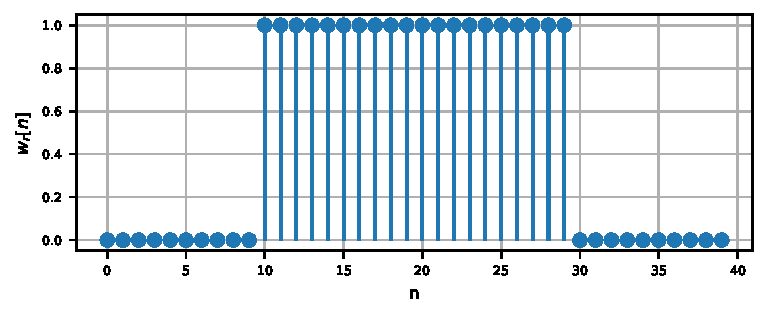
\includegraphics[width=.45\linewidth]{papers/sonogramm/images/rect_time.pdf}}
%     \qquad
%     \subfigure[Frequenzspektrum des Rechtecksfenster von Abbildung \ref{sonogramm:recttime}
%          mit einer Abtastfrequenz von 20 Hz. \label{sonogramm:rectfreq}]
%       {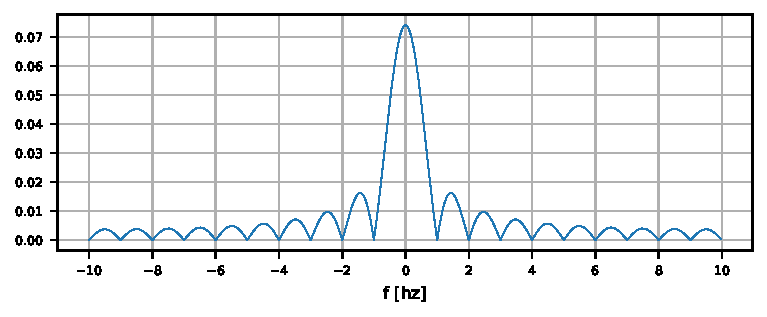
\includegraphics[
%         width=.45\linewidth
%         % scale = 1.2,
%         % trim = 0 40 0 0, clip,
%       ]{papers/sonogramm/images/rect_freq.pdf}}
%     \caption{
%         Frequenzanalyse eines Rechteckfensters. In (b)
%         sieht man die Nulldurchgänge bei vielfachen von $1/T$.
%     }
% \end{figure}
% \begin{figure}
%     \centering
%     \begin{subfigure}
%         \centering
%         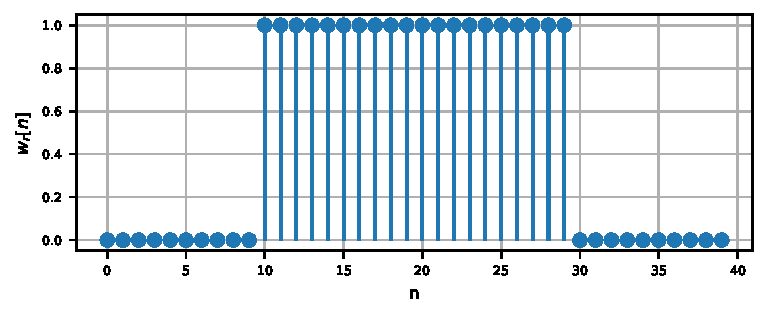
\includegraphics[width=1\linewidth]{papers/sonogramm/images/rect_time.pdf}
%         \caption{Rechtecksfenster mit $L_w = 20$ und T = 1 Sekunde.}
%         \label{sonogramm:recttime}
%     \end{subfigure}
%     \hfill
%     \begin{subfigure}
%         \centering
%         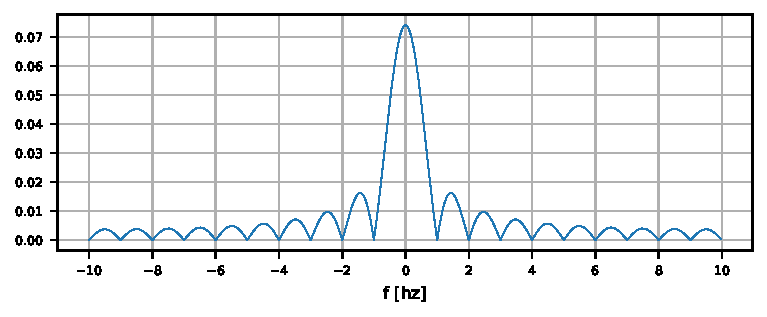
\includegraphics[width=1\linewidth]{papers/sonogramm/images/rect_freq.pdf}
%         \caption{Frequenzspektrum des Rechtecksfenster von Abbildung \ref{sonogramm:recttime}
%         mit einer Abtastfrequenz von 20 Hz.}
%         \label{sonogramm:rectfreq}
%     \end{subfigure}
%     \label{fig:three graphs}
%        \caption{Frequenzanalyse eines Rechteckfensters. In Abbildung \ref*{sonogramm:rectfreq}
%        sieht man die Nulldurchgänge bei vielfachen von $1/T$.}

% \end{figure}
\begin{figure}
    \centering
    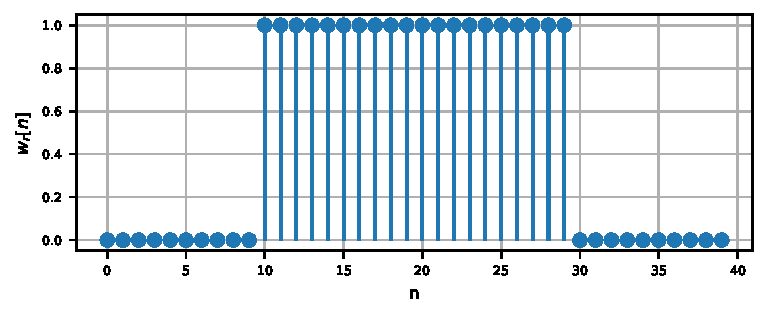
\includegraphics{papers/sonogramm/images/rect_time.pdf}
    \caption{Rechtecksfenster mit $L_w = 20$.
    \label{sonogramm:recttime}
    }
\end{figure}

\begin{figure}
    \centering
    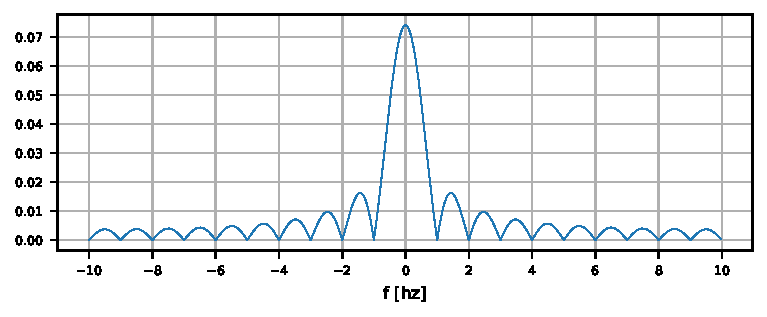
\includegraphics{papers/sonogramm/images/rect_freq.pdf}
    \caption{Frequenzspektrum des Rechtecksfenster von Abbildung \ref{sonogramm:recttime}
    mit einer Abtastfrequenz von 20 Hz. Die Nulldurchgänge sind jeweils bei ganzzahligen Vielfachen
    von $1/T$.
    \label{sonogramm:rectfreq}
    }
\end{figure}
TODO Grafik

\subsection{Rechnerische Auflösung}
Bei einer DFT werden so viele Frequenzsamples berechnet wie das
Zeitsignal hat. 
TODO alot

\subsection{Fensterfunktion}
Der Faltungssatz beschreibt 
\begin{align}
    f(t) * g(t)& \xrightarrow{\mathscr{F}} F(\omega)G(\omega),\\
    f(t) g(t)&\xrightarrow{\mathscr{F}}F(\omega) * G(\omega).
\end{align}
Das bedeutet, das die Verwendung von Fensterfunktionen das Frequenzspektrum
des Signals durch eine Faltung verschmieren.
\subsection{Überlappung}
TODO Alles


